\section{Introduction} 
% Section outline:
% Overall summary of project - ~1 sentence per major goal
% ~1 Paragraph for each major goal
% Paragraph at end describing what is in this document

%TODO: Say that RBE3001 is a course at WPI

The goal of this project was to create an adaptable control system whose purpose is to drive a variety of robotic arms. To prove the usefulness of our system, we retrofitted an existing robot arm from the RBE 3001 course with our control system.  In addition to this, we modified the existing arm to include an interchangeable joint on the end of our arm, controlled by our system. To interface with our system, we created a GUI for easy configuration and basic control of the arm. The base communicates with a computer running control code through the software application. \\
\newline

\begin{figure}[H]
\centering
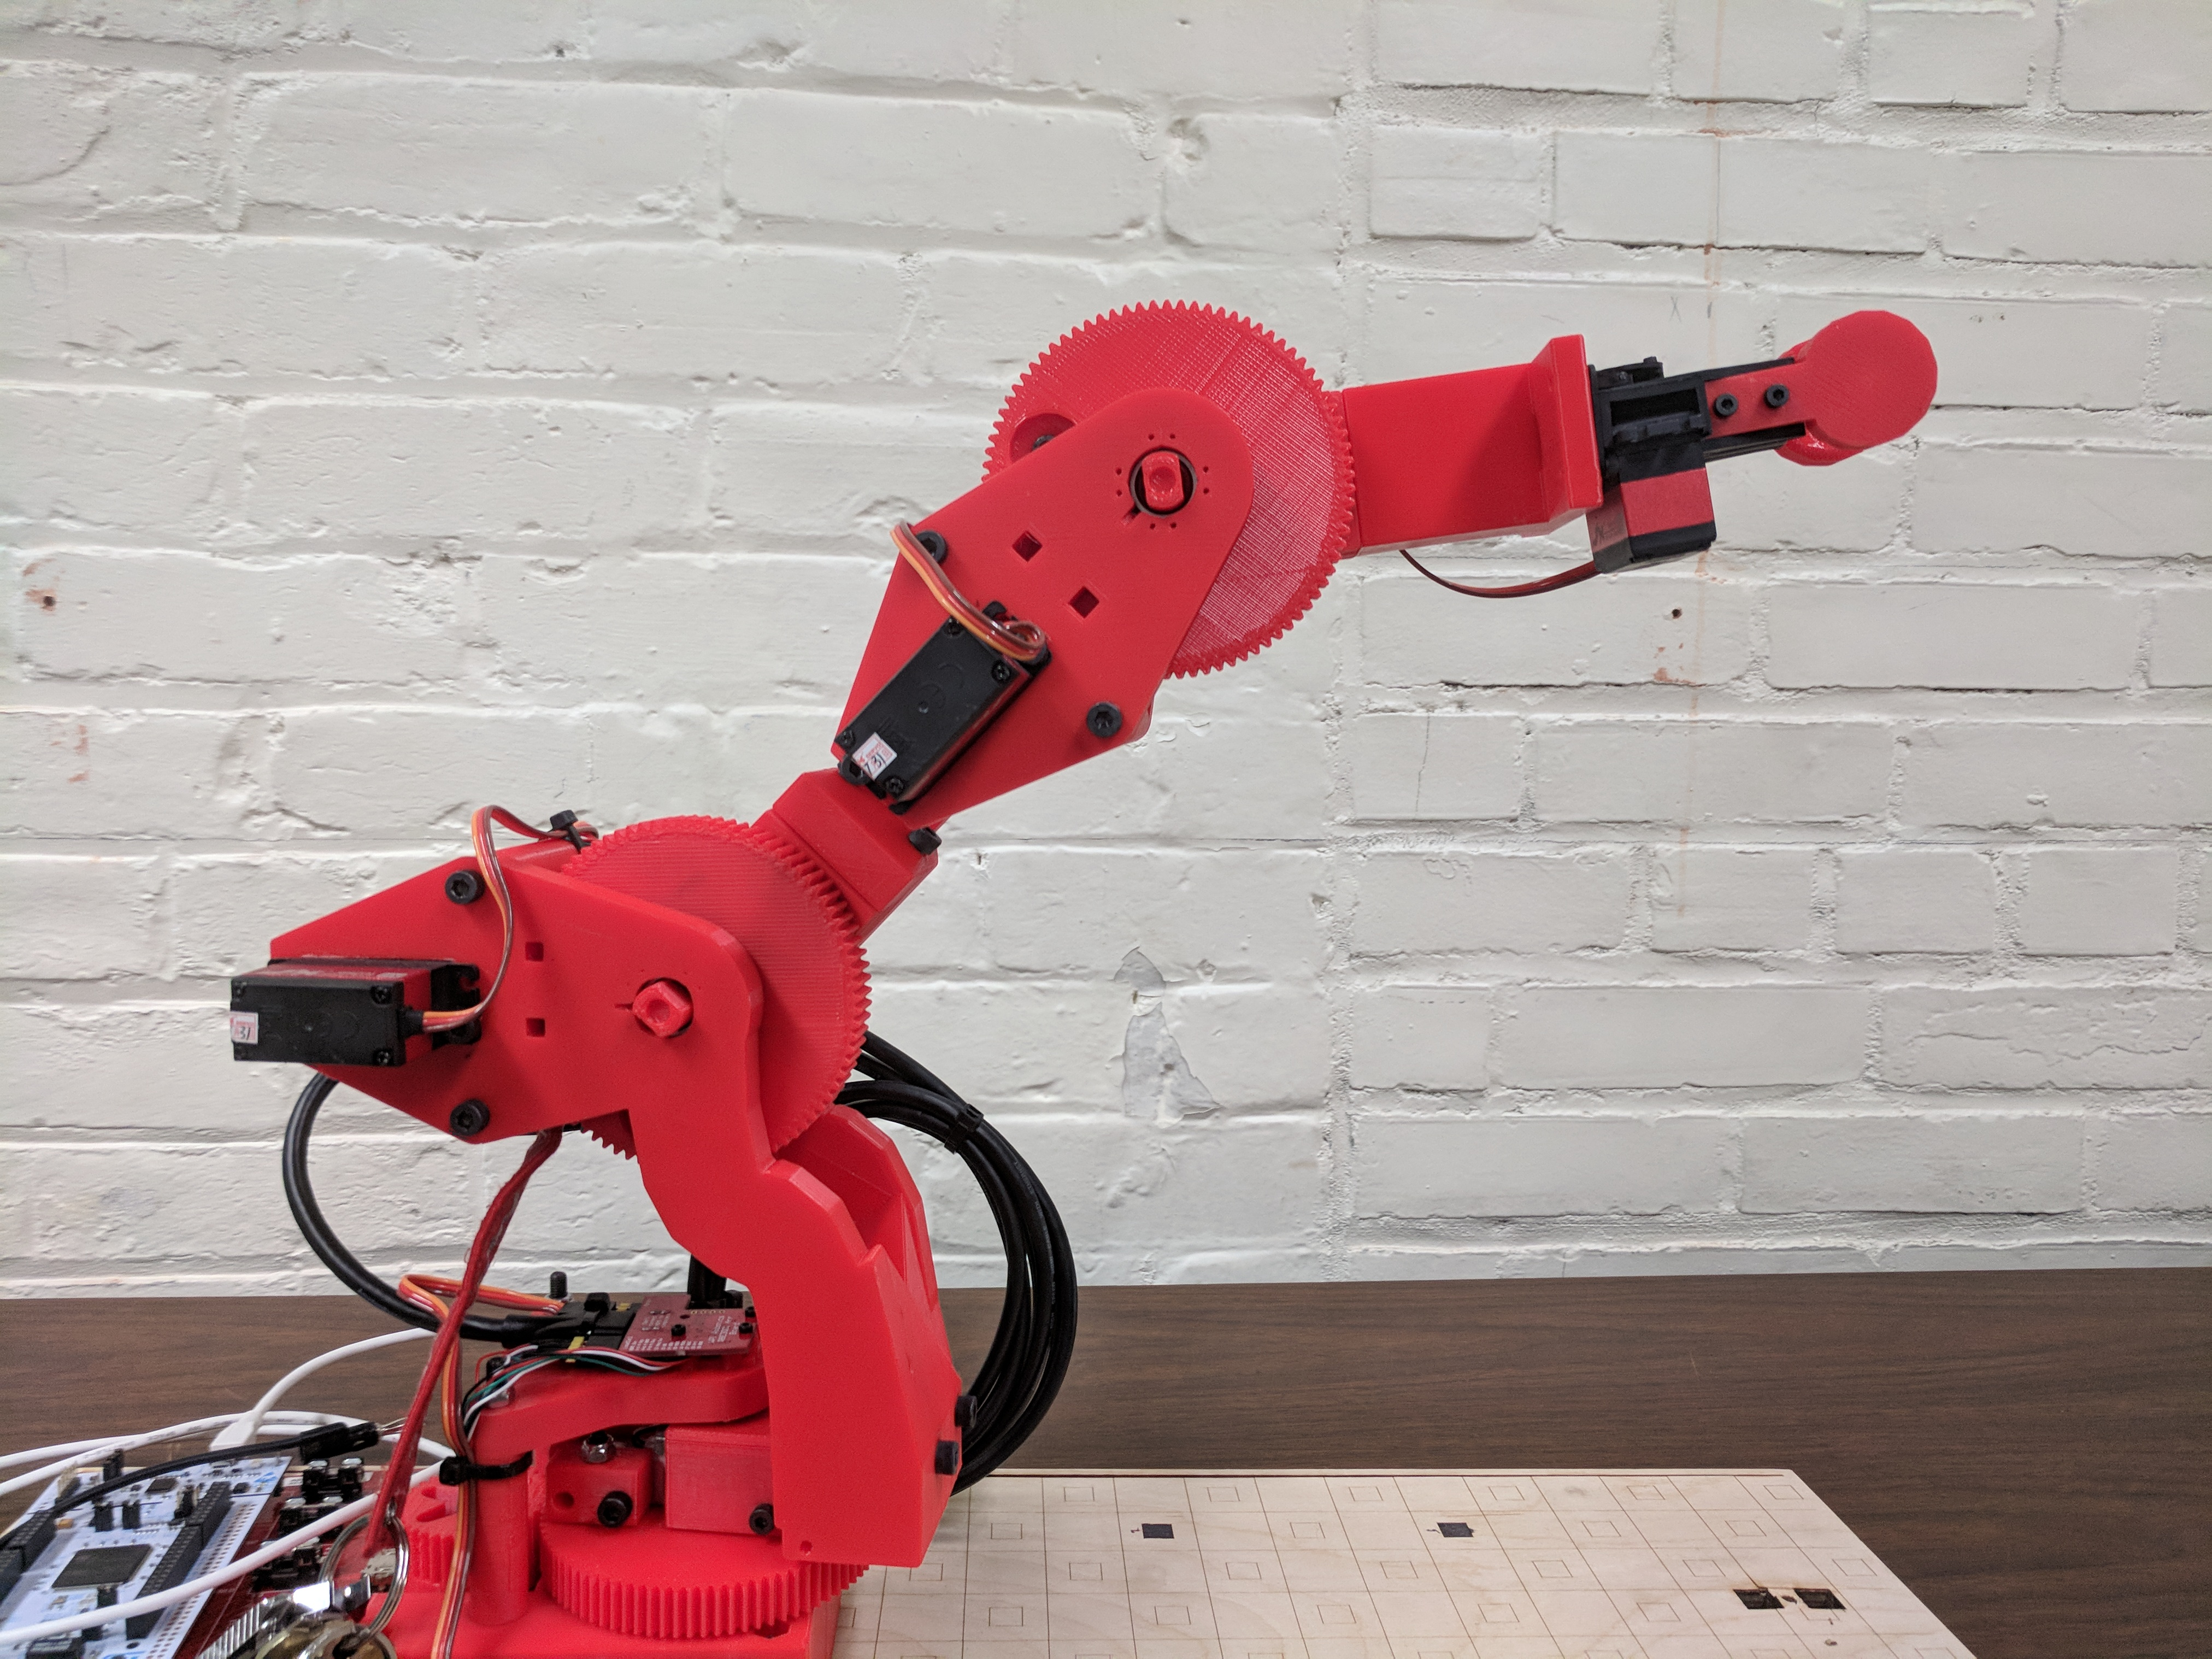
\includegraphics[width=\textwidth]{Initial_3001_Arm}
\caption{Unmodified RBE 3001 Arm}
\label{fig:Functional_Block_Diagram}
\end{figure}

\newline
The existing RBE 3001 arm already has its own central control system. We removed this and replaced it with our own distributed one. To accomplish this, we designed a joint control board that communicates with a base controller.  We also designed and implemented a new joint on the arm. This new joint is interchangeable to prove that our software and control system will work with more than one configuration. The joint implements our control board. \\


\newline
We created a software application to interface with a constructed arm. The user inputs how they have configured their arm into this application and are then able to do some simple control. Another feature of this application is the ability to record a series of poses for the arm to perform. In addition to this software, we also created some programming libraries to allow users to control the arm with their own programs. \\
\newline
In this document, we will outline some existing robot arms and highlight the differences between these arms and our arm. We then discuss what work there is to be done on this project. After discussing the work to be done, we state how this work will satisfy the capstone design requirements for each of the three disciplines represented by our group members. Then, we state the constraints we expect going forward with this project. Next, the acceptance criteria for any deliverables at the end of this project will be outlined. 
